\fancyhead{}
\fancyfoot{}

\newtheorem{teorema}{Teorema}

%\pagestyle{fancy}
\pagestyle{plain}
\lhead{Conceptos fundamentales, teoría y antecedentes}

\chapter{Conceptos fundamentales, teoría y antecedentes}

En este capítulo se desarrolla el marco teórico conceptual y referencial de este trabajo de investigación. En primer lugar, se presentan las definiciones básicas asociadas al estudio, como las relacionadas con la tecnología de geolocalización y radiofrecuencia. Por último, se presentan los antecedentes de trabajos anteriormente realizados en el área sobre el cual está basado este trabajo final de grado.


\section{Inteligencia Artificial}
\subsection{Evolución histórica}
La inteligencia artificial (IA) tiene sus orígenes en los trabajos pioneros de Alan Turing, quien en 1950 publicó su artículo ``\textit{Computing Machinery and Intelligence}'' donde propuso el ahora famoso \textit{Test} de Turing como método para evaluar la capacidad de una máquina para exhibir un comportamiento inteligente. El término ``Inteligencia Artificial'' fue acuñado formalmente en 1956 durante la conferencia de Dartmouth, organizada por John McCarthy, Marvin Minsky, Nathaniel Rochester y Claude Shannon, estableciendo así el nacimiento de este campo como disciplina académica \cite{turing1950}.

Las décadas de 1960 y 1970 vieron el desarrollo de los primeros sistemas expertos como \textit{DENDRAL} y \textit{MYCIN}, que demostraron la capacidad de las computadoras para simular el razonamiento humano en dominios específicos. Sin embargo, las limitaciones técnicas y teóricas condujeron a lo que se conoce como el ``invierno de la IA'' en los años 80, un período de reducción de financiación e interés en la investigación \cite{feigenbaum1988}.

El resurgimiento de la IA comenzó en los años 90 con avances en \textit{machine learning}, particularmente con el desarrollo de métodos estadísticos y probabilísticos. El verdadero punto de inflexión llegó en 2012, cuando una red neuronal profunda desarrollada por Krizhevsky et al. redujo drásticamente la tasa de error en el desafío de reconocimiento visual \textit{ImageNet}, inaugurando la era moderna del \textit{deep learning} \cite{krizhevsky2012}.

\subsection{Concepto de inteligencia artificial}
La IA puede ser definida desde cuatro perspectivas diferentes: sistemas que piensan como humanos, sistemas que actúan como humanos, sistemas que piensan racionalmente y sistemas que actúan racionalmente. Esta multidimensionalidad refleja la complejidad inherente al campo \cite{russell2020}.

La IA es la capacidad de un sistema para interpretar correctamente datos externos, aprender de dichos datos y utilizar esos aprendizajes para lograr objetivos y tareas específicas mediante adaptación flexible. Esta definición enfatiza las capacidades de aprendizaje y adaptación que caracterizan a los sistemas de IA modernos \cite{kaplan2019}.

La inteligencia artificial representa la convergencia de diversos campos como la computación, la estadística, la neurociencia y la psicología cognitiva, con el objetivo de crear sistemas capaces de realizar tareas que normalmente requieren inteligencia humana, incluyendo el aprendizaje, la resolución de problemas, el reconocimiento de patrones y la toma de decisiones en entornos complejos y dinámicos.

\subsection{Modelos de Inteligencia Artificial}
La IA puede clasificarse en IA estrecha o débil (diseñada para tareas específicas), IA general (capaz de realizar cualquier tarea intelectual humana) e IA superinteligente (hipotética, superaría la inteligencia humana). Actualmente, todos los sistemas desplegados son ejemplos de IA estrecha, aunque la investigación avanza hacia desarrollos más generales \cite{bostrom2014}.

\section{\textit{YOLO} (\textit{You Only Look Once})}

\subsection{Concepto}
\textit{YOLO} es un sistema de detección de objetos en tiempo real que procesa imágenes completas en una sola evaluación de red neuronal, dividiendo la imagen en regiones y prediciendo simultáneamente cuadros delimitadores y probabilidades de clase para cada región \cite{yolo_site}.

\textit{YOLO} es un enfoque unificado para la detección de objetos que trata la detección como un problema de regresión espacial, donde una única red neuronal predice directamente cuadros delimitadores y probabilidades de clase simultáneamente. Este diseño posibilita una optimización directa de extremo a extremo y posibilita la detección en tiempo real mientras mantiene alta precisión \cite{yolo_paper}.

\subsection{Características}
\textit{YOLO} destaca por su velocidad de procesamiento, alcanzando 45 fotogramas por segundo en su configuración base y hasta 155 fotogramas por segundo en su versión más rápida, lo que posibilita aplicaciones en tiempo real. Su arquitectura unificada optimiza directamente el rendimiento de detección al tratar la detección como un problema de regresión único \cite{bochkovskiy2020}.

La arquitectura de \textit{YOLO} divide la imagen de entrada en una cuadrícula S×S y, para cada celda de la cuadrícula, predice B cuadros delimitadores junto con sus puntuaciones de confianza y probabilidades de clase. Esta formulación posibilita al modelo considerar simultáneamente características visuales globales y contexto espacial, contribuyendo a su capacidad para generalizar bien a nuevas situaciones y dominios \cite{yolo_docs}.

\subsection{Arquitectura de YOLOv11}

La arquitectura de {YOLOv11 sigue el paradigma modular \textit{backbone}--\textit{neck}--\textit{head}, optimizado para lograr un alto rendimiento en tareas de detección de objetos en tiempo real. Desarrollado por Ultralytics, este modelo introduce mejoras en la extracción de características, mecanismos de atención y predicción multi-escala que permiten mantener una elevada precisión (\textit{mAP}) sin comprometer la velocidad de inferencia, incluso en entornos con recursos computacionales limitados \cite{analyticsvidhya2025}.

\textbf{Backbone – Extracción de características}

El \textit{backbone} de YOLOv11 emplea una arquitectura tipo \textit{DarkNet/DarkFPN} para extraer tres niveles de características (P3, P4 y P5), representando patrones visuales desde detalles finos hasta información semántica de alto nivel. Incorpora bloques optimizados para eficiencia computacional y culmina con el módulo \textit{SPPF (Spatial Pyramid Pooling Fast)}, que fusiona información de contexto a múltiples escalas mediante \textit{max-pooling}, mejorando la detección de objetos pequeños sin degradar el rendimiento en tiempo real.

\textbf{Neck – Fusión y atención espacial}

El \textit{neck} está diseñado para combinar y refinar las características extraídas en el \textit{backbone}. YOLOv11 introduce el bloque \textit{C2PSA (Cross Stage Partial con Spatial Attention)}, que aplica atención espacial en sub-rutas parciales del flujo de datos, destacando regiones relevantes y atenuando el ruido. Posteriormente, se emplea un esquema tipo FPN con \textit{upsampling} y concatenación para mantener la coherencia entre distintas resoluciones, optimizando así la detección en múltiples escalas con un coste computacional controlado.

\textbf{Head – Predicción multi-escala}

El \textit{head} opera sobre los tres mapas de características (P3, P4, P5) generados tras el \textit{neck}, permitiendo detectar objetos pequeños, medianos y grandes de forma simultánea. Cada salida genera predicciones de cajas delimitadoras y categorías, ajustadas según el \textit{stride} correspondiente. En la etapa final de inferencia se aplican algoritmos de \textit{Non-Maximum Suppression (NMS)} para eliminar detecciones redundantes y conservar las más probables.

\vspace*{-0.5 cm}


\begin{figure}[H]
\leavevmode
\begin{minipage}{\textwidth}
\begin{center}
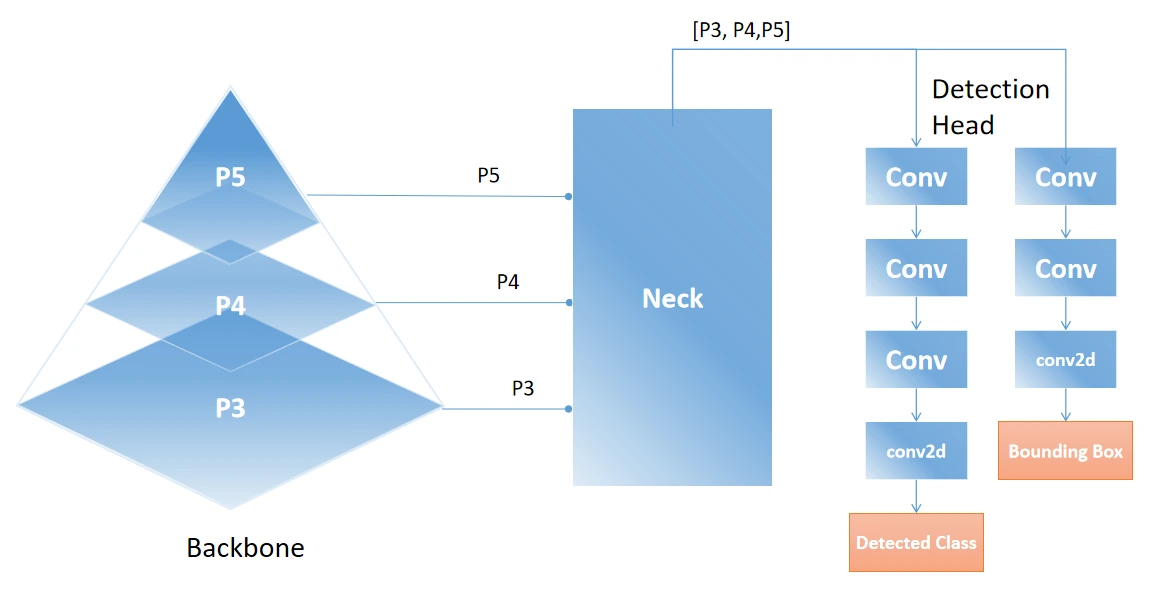
\includegraphics[width=0.8\textwidth]{./capitulo_02/figures/yolo11}
\caption{\textit{Diagrama de flujo del modelo YOLO}. \label{fig:yolo11}}
\end{center}
\end{minipage}
\end{figure}

\subsection{Arquitectura de YOLOv12}

\textit{YOLOv12} es una evolución de la familia \textit{YOLO} que integra mecanismos de atención en un modelo que mantiene la rapidez característica de los detectores basados en \emph{CNN} (redes convolucionales). Su diseño busca balancear precisión y velocidad, superando las limitaciones tradicionales de los mecanismos de atención, que suelen ser lentos y consumir mucha memoria. \cite{learnopencv2025}.


\textbf{Módulo de Atención por Áreas (\emph{Area Attention Module} - A2)}

\begin{itemize}
    \item Divide el mapa de características en segmentos locales, en lugar de aplicar atención global costosa.
    \item Este método conserva un campo receptivo grande (aunque menor que la atención global) pero con una complejidad computacional mucho menor.
    \item Gracias a esta división sencilla (reorganización del tensor) se reduce el costo computacional a la mitad, acelerando el proceso sin perder precisión significativa.
\end{itemize}

\textbf{Redes de Agregación Residual Eficiente (\emph{Residual Efficient Layer Aggregation Networks} - R-ELAN)}

\begin{itemize}
    \item Evolución del módulo \emph{ELAN} usado en YOLO anteriores, que mejora la agregación de características.
    \item Introduce conexiones residuales a nivel de bloque con un factor de escala para estabilizar el entrenamiento y evitar problemas de convergencia, especialmente con atención.
    \item Cambia la forma de agregar características, usando un solo mapa de características procesado mediante bloques tipo \emph{cuello de botella} para mejorar eficiencia y rendimiento.
\end{itemize}

\textbf{Mejoras Arquitectónicas}

\begin{itemize}
    \item \textbf{\emph{Flash Attention}:} Optimiza el acceso a memoria para acelerar la atención, cerrando la brecha de velocidad entre atención y convoluciones.
    \item \textbf{Eliminación del \emph{Codificado Posicional}:} Se suprime el uso de codificaciones posicionales explícitas en la atención para simplificar y acelerar el modelo sin perder precisión.
    \item \textbf{Ajuste en la Expansión del \emph{MLP}:} Reduce la relación de expansión del perceptrón multicapa de 4 a 1.2 para equilibrar la carga computacional entre atención y redes \emph{feed-forward}.
    \item \textbf{Reducción de la Profundidad de Bloques:} Disminuye la cantidad de bloques apilados en la última etapa para facilitar la optimización y mejorar la velocidad de inferencia.
    \item \textbf{Uso Extensivo de Operadores Convolucionales:} Prefiere convoluciones con normalización por lotes en lugar de capas lineales con normalización de capas, aprovechando su eficiencia computacional.
\end{itemize}

\textbf{Resultados}

\begin{itemize}
    \item YOLOv12 mejora la precisión (\emph{mAP}) respecto a versiones anteriores (YOLOv10, YOLOv11) y supera a otros modelos recientes, manteniendo o mejorando la velocidad de inferencia.
    \item Estas mejoras son escalables para distintos tamaños de modelo (desde versiones pequeñas a grandes).
    \item Sin embargo, para obtener la máxima velocidad, YOLOv12 requiere GPUs modernas que soporten \emph{Flash Attention} (arquitecturas NVIDIA Turing en adelante).
\end{itemize}




\begin{figure}[H]
\leavevmode
\begin{minipage}{\textwidth}
\begin{center}
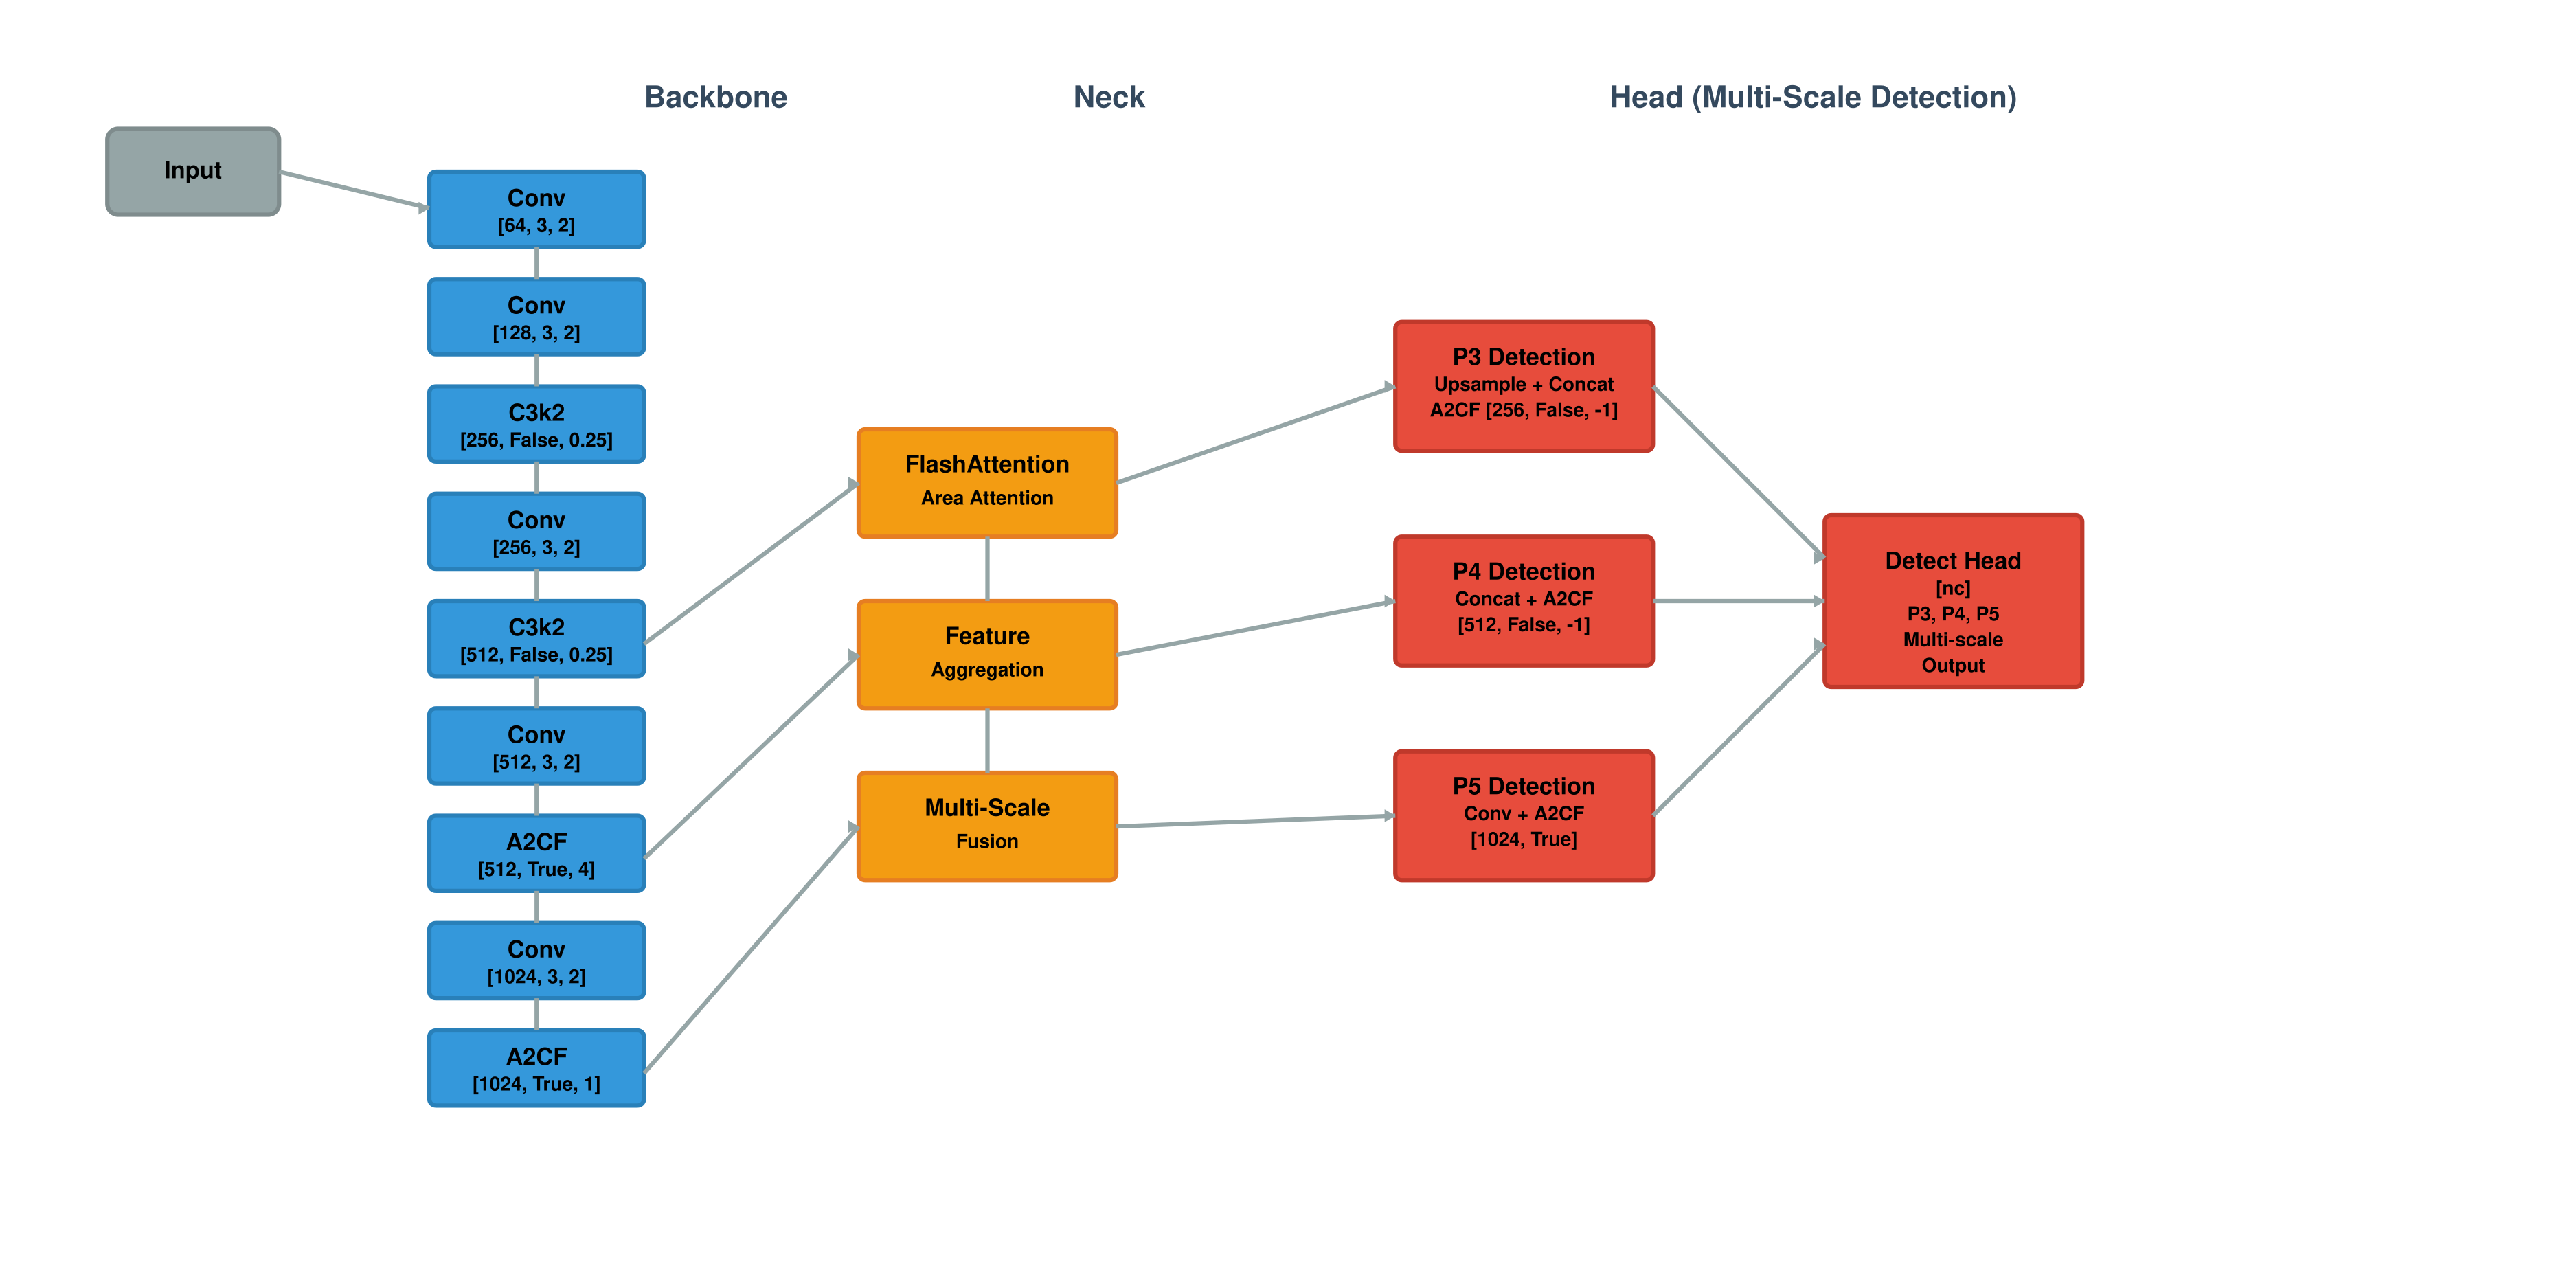
\includegraphics[width=1.2\textwidth]{./capitulo_02/figures/yolo12}
\caption{\textit{Diagrama de flujo del modelo YOLO – versión completa}. \label{fig:yolo12}}
\end{center}
\end{minipage}
\end{figure}

\section{Visión por Computadora}
\subsection{Evolución histórica}
La visión por computadora como disciplina formal comenzó a desarrollarse en los años 60, cuando investigadores como Larry Roberts exploraron la posibilidad de reconstruir objetos 3D a partir de imágenes 2D en su tesis doctoral del \textit{MIT}. Durante la década siguiente, David Marr estableció un marco teórico influyente que conceptualizaba la visión como un proceso de información multinivel \cite{szeliski2022}.

\subsection{Concepto}
La visión por computadora es la construcción de descripciones explícitas y significativas de objetos físicos a partir de imágenes. Esta disciplina busca dotar a las máquinas de la capacidad de interpretar y comprender información visual de manera similar a la visión humana \cite{forsyth2021}.

\subsection{Fases de un Sistema de Visión por Computadora}

Un sistema de visión por computadora se estructura desde la adquisición de datos visuales hasta la interpretación de los resultados. Estas fases conforman un flujo modular, donde cada una contribuye de manera específica al procesamiento automatizado de imágenes. La correcta definición e implementación de estas fases es esencial para garantizar la eficiencia, precisión y trazabilidad del sistema \cite{szeliski2022}.

\textbf{Adquisición de Imágenes:} La primera fase consiste en la obtención de imágenes digitales a través de sensores o dispositivos de captura. Esto puede incluir cámaras digitales, dispositivos móviles, escáneres, sensores térmicos, tomografías computarizadas o equipos de rayos X. El resultado es una imagen digital en formato estándar (por ejemplo, \textit{PNG}, \textit{JPEG} o \textit{DICOM}), que servirá como entrada para las fases posteriores del sistema \cite{wang2020}.

La calidad de la imagen capturada incide directamente en la efectividad del análisis visual. Por ello, durante esta fase también pueden realizarse tareas de conversión de formato, validación de resolución y verificación de parámetros como la nitidez, exposición y escala, garantizando así una base adecuada para los procesos siguientes \cite{gonzalez2018}.

\textbf{Preprocesamiento:} El preprocesamiento de imágenes tiene como finalidad mejorar la calidad visual y estandarizar las características técnicas de las imágenes antes de su análisis. Esta fase no altera el contenido semántico, pero sí lo optimiza, eliminando interferencias que podrían afectar negativamente la precisión del sistema \cite{jain2021}. Entre las técnicas más comunes se incluyen:

\begin{itemize}
  \item \textit{Redimensionamiento:} ajustar todas las imágenes a dimensiones uniformes compatibles con el modelo.
  \item \textit{Normalización:} escalar los valores de los píxeles a un rango determinado (por ejemplo, de 0 a 1).
  \item \textit{Reducción de ruido:} aplicación de filtros como el gaussiano o de mediana.
  \item \textit{Mejoramiento de contraste:} mediante técnicas como la ecualización del histograma.
  \item \textit{Alineación o rotación:} estandarizar la orientación de las imágenes.
\end{itemize}

Estas operaciones preparan las imágenes para su procesamiento eficiente, posibilitando que los algoritmos se enfoquen en patrones estructurales relevantes.

\textbf{Segmentación y Extracción de Características:} La tercera fase implica dos procesos complementarios:

\begin{itemize}
  \item \textit{Segmentación:} consiste en dividir la imagen en regiones homogéneas o de interés, separando estructuras relevantes del fondo \cite{shapiro2021}.
  \item \textit{Extracción de características:} convierte dichas regiones en representaciones numéricas o vectores de atributos que puedan ser utilizados por algoritmos de clasificación \cite{nixon2020}.
\end{itemize}

Las características extraídas pueden ser geométricas (forma, contorno, área), texturales (rugosidad, patrones repetitivos), colorimétricas (intensidad, distribución tonal) o espaciales (posición y relación con otras regiones). El éxito de esta fase depende de la pertinencia de los atributos seleccionados, ya que determinan el rendimiento del modelo en la siguiente etapa.

\textbf{Clasificación o Detección:} En esta fase se aplican modelos de inteligencia artificial para identificar, clasificar o detectar automáticamente patrones presentes en las imágenes \cite{lecun2015}. La elección del modelo depende del objetivo del sistema: si se desea clasificar una imagen completa o localizar múltiples objetos específicos dentro de ella \cite{krizhevsky2017}.

\textbf{Interpretación y Salida del Sistema:} En la última fase, los resultados obtenidos por el modelo son traducidos a un formato comprensible y útil para el usuario o sistema final. Esta fase implica la visualización de resultados, generación de informes y la toma de decisiones basada en la interpretación de los datos procesados \cite{forsyth2021}.

\section{Radiografías}
Las radiografías son una técnica de imagen médica que utiliza rayos X para visualizar las estructuras internas del cuerpo. Funcionan mediante la emisión de radiación electromagnética de alta energía que atraviesa el cuerpo y es absorbida en diferentes grados según la densidad de los tejidos \cite{bushberg2021essential}. Estas diferencias de absorción crean un patrón de sombras que se registra en un detector, generando una imagen bidimensional donde las estructuras densas como los huesos aparecen más claras (radiopacas) y las menos densas como el aire aparecen más oscuras (radiolúcidas) \cite{carlton2020principles}.

Las radiografías siguen siendo una herramienta diagnóstica fundamental en medicina debido a su accesibilidad, rapidez, bajo costo relativo y capacidad para proporcionar información anatómica esencial. Son ampliamente utilizadas para examinar fracturas óseas, evaluar alteraciones estructurales en órganos internos, detectar cuerpos extraños y diagnosticar diversas condiciones patológicas.

La tecnología radiográfica ha evolucionado desde las placas fotográficas tradicionales hasta los sistemas digitales modernos, que posibilitan el procesamiento, almacenamiento y transmisión electrónica de imágenes, facilitando el análisis asistido por computadora y la aplicación de técnicas de inteligencia artificial para mejorar la precisión diagnóstica.


\section{Fracturas óseas}
Las fracturas óseas representan interrupciones en la continuidad estructural de un hueso, producidas cuando las fuerzas aplicadas superan la resistencia del tejido óseo \cite{nauth2020fracture}. Radiográficamente, se manifiestan como líneas radiolúcidas (oscuras) que atraviesan la estructura ósea, a menudo acompañadas de desplazamiento de fragmentos, cambios en la alineación anatómica y, en casos agudos, edema de tejidos blandos circundantes \cite{browner2019skeletal}.

El diagnóstico radiográfico de fracturas requiere la identificación de signos directos (línea de fractura, desplazamiento) e indirectos (reacción perióstica, edema). Las radiografías convencionales siguen siendo la modalidad de imagen de primera línea para la evaluación inicial de fracturas, aunque en casos complejos pueden requerir técnicas avanzadas como tomografía computarizada o resonancia magnética.

Las fracturas pueden clasificarse según múltiples criterios: por su comunicación con el exterior (cerradas o abiertas), por su patrón (transversales, oblicuas, espirales, conminutas), por su localización anatómica o por el mecanismo de lesión subyacente. El diagnóstico preciso y la correcta clasificación son esenciales para determinar el tratamiento adecuado y predecir el pronóstico.

\section{Diagnóstico por imágenes en veterinaria}
El diagnóstico por imágenes en medicina veterinaria comprende un conjunto de técnicas no invasivas que posibilitan visualizar las estructuras anatómicas internas de los animales con fines diagnósticos y terapéuticos. La radiografía convencional constituye el pilar fundamental de esta disciplina, particularmente en la evaluación del sistema musculoesquelético canino, donde posibilita la detección de fracturas, luxaciones, neoplasias óseas y alteraciones articulares degenerativas \cite{thrall2018textbook}.

En el contexto veterinario, la interpretación radiográfica presenta desafíos específicos relacionados con la variabilidad anatómica entre razas caninas, las limitaciones en el posicionamiento del paciente y la necesidad frecuente de sedación. La radiología digital ha transformado significativamente esta práctica al mejorar la calidad de imagen, reducir la exposición a radiación y facilitar el almacenamiento y transmisión de estudios \cite{mattoon2021digital}.


\section{Anatomía Ósea Canina}

El sistema esquelético canino presenta características anatómicas específicas que difieren del esquelético humano, tanto en proporciones como en funcionalidad. Los perros poseen aproximadamente 319 huesos, variando según la raza y el tamaño \cite{dyce2012anatomia}. En esta investigación se analizaron cuatro tipos principales de huesos que representan las estructuras óseas más comúnmente afectadas por fracturas traumáticas en la práctica veterinaria.

\begin{figure}[H]
\leavevmode
\begin{minipage}{\textwidth}
\begin{center}
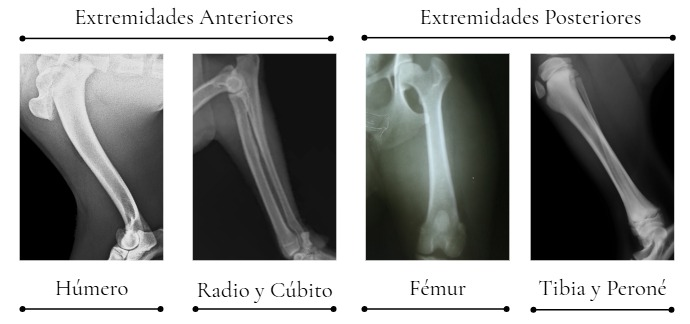
\includegraphics[width=1\textwidth]{./capitulo_02/figures/Tipos_de_Huesos}
\caption{\textit{Tipos de huesos en extremidades caninas}. \label{fig:tipos_huesos}}
\end{center}
\end{minipage}
\end{figure}

\subsection{Húmero}

El húmero constituye el hueso principal de la extremidad anterior canina, ubicado entre la escápula y el antebrazo \cite{hermanson2019millers}. Incluye cabeza humeral, tuberosidades mayor y menor, y región distal con cóndilos humerales como características anatómicas relevantes. Las fracturas humerales son frecuentes en perros jóvenes y activos, representando aproximadamente el 8-12\% de todas las fracturas de huesos largos \cite{fossum2021small}.

\subsection{Radio y Cúbito}

El radio y cúbito forman el esqueleto del antebrazo canino, estando más fusionados funcionalmente que en otros mamíferos \cite{dyce2012anatomia}. El radio es el hueso principal de carga mientras el cúbito proporciona estabilidad articular y puntos de inserción muscular. Las fracturas de radio-cúbito son comunes en razas pequeñas y representan el 8-18\% de todas las fracturas en perros \cite{johnson2018fundamentals}.

\subsection{Fémur}

El fémur es el hueso más largo y fuerte de la extremidad posterior del perro, extendiéndose desde la cadera hasta la rodilla \cite{hermanson2019millers}. Presenta cabeza femoral, cuello femoral, trocánteres mayor y menor, y diáfisis como estructuras principales. Las fracturas femorales representan aproximadamente el 20-25\% de todas las fracturas óseas en la práctica veterinaria \cite{piermattei2016handbook}.

\subsection{Tibia y Peroné}

La tibia y peroné constituyen el esqueleto de la pierna canina, siendo la tibia el hueso principal de soporte del peso corporal \cite{hermanson2019millers}. La tibia presenta una cresta tibial prominente para inserción del ligamento rotuliano y los músculos extensores. El peroné, más delgado, proporciona estabilidad articular y puntos de inserción muscular específicos \cite{tobias2017veterinary}.

\section{Clasificación de Fracturas}

El sistema de diagnóstico desarrollado identifica cinco tipos principales de fracturas basándose en las características morfológicas observables en imágenes radiográficas caninas, siguiendo los principios de clasificación AO modificados para medicina veterinaria \cite{unger2024ao}.

\begin{figure}[H]
\leavevmode
\begin{minipage}{\textwidth}
\begin{center}
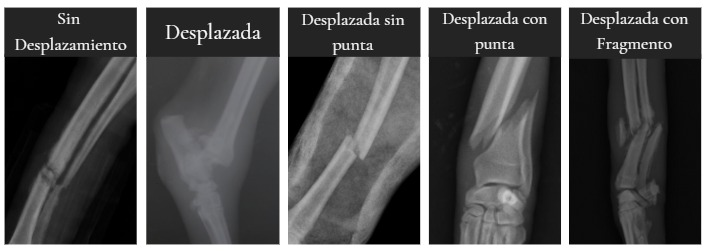
\includegraphics[width=1\textwidth]{./capitulo_02/figures/Tipos_de_Fracturas}
\caption{\textit{Tipos de fracturas óseas caninas según clasificación morfológica}. \label{fig:tipos_fracturas}}
\end{center}
\end{minipage}
\end{figure}

\subsection{Sin Desplazamiento}

Fracturas en las que los fragmentos óseos mantienen su alineación anatómica normal con separación mínima (menos de 2mm) \cite{piermattei2016handbook}. La línea de fractura es visible radiográficamente pero no existe separación significativa entre los fragmentos. Este tipo de fractura generalmente presenta mejor pronóstico y menor tiempo de consolidación.

\subsection{Desplazada}

Fracturas caracterizadas por la pérdida de alineación entre los fragmentos óseos principales con separación superior a 2mm o angulación visible \cite{fossum2021small}. Los segmentos fracturados muestran separación, angulación o cabalgamiento visible en las proyecciones radiográficas estándar.

\subsection{Desplazada sin Punta}

Fracturas desplazadas donde los fragmentos principales presentan bordes relativamente lisos sin formación de fragmentos triangulares o puntiagudos \cite{johnson2018fundamentals}. Este patrón facilita la reducción quirúrgica y presenta menor riesgo de complicaciones de tejidos blandos.

\subsection{Desplazada con Punta}

Fracturas que combinan desplazamiento con la presencia de fragmentos óseos de morfología triangular o puntiaguda \cite{tobias2017veterinary}. Estos fragmentos puntiagudos son fácilmente identificables en las imágenes radiográficas y pueden causar lesiones de tejidos blandos adyacentes.

\subsection{Desplazada con Fragmento}

Fracturas caracterizadas por desplazamiento de los fragmentos principales acompañado de fragmentos óseos adicionales de diversos tamaños \cite{piermattei2016handbook}. Representa el patrón más complejo de fractura en términos de número de fragmentos y requiere técnicas de fijación más sofisticadas.

\section{Localización Anatómica}

La ubicación de la fractura dentro del hueso se clasifica en tres regiones principales que determinan las características biomecánicas, el pronóstico de la lesión y el método de tratamiento más apropiado \cite{markel2019biomechanics}.

\begin{figure}[H]
\leavevmode
\begin{minipage}{\textwidth}
\begin{center}
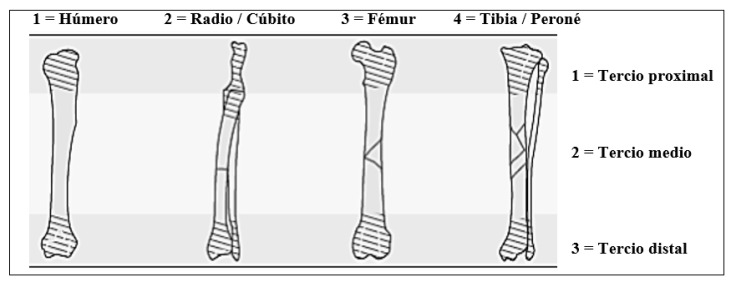
\includegraphics[width=1\textwidth]{./capitulo_02/figures/Ubicacion_de_la_Fractura}
\caption{\textit{Ubicación de la fractura en el esqueleto canino según regiones anatómicas}. \label{fig:ubicacion_fractura}}
\end{center}
\end{minipage}
\end{figure}

\subsection{Tercio Proximal}

Región que comprende el extremo del hueso más cercano al tronco del animal \cite{dyce2012anatomia}. Incluye las estructuras articulares proximales, áreas de inserción de los principales grupos musculares y zonas de alta vascularización. Las fracturas en esta región frecuentemente involucran componentes articulares.

\subsection{Tercio Medio}

Corresponde a la diáfisis o cuerpo central del hueso largo \cite{hermanson2019millers}. Esta región se caracteriza por su cortical gruesa y representa la principal área de soporte estructural del hueso. Las fracturas diafisarias tienen generalmente buen pronóstico de consolidación debido a la rica vascularización perióstica.

\subsection{Tercio Distal}

Región que abarca el extremo del hueso más alejado del tronco \cite{hermanson2019millers}. Frecuentemente incluye componentes articulares distales y estructuras importantes para la biomecánica articular. Requiere reducción anatómica precisa para mantener la función articular normal \cite{thrall2018textbook}.

\section{Aplicación web}
Una aplicación web constituye un \textit{software} alojado en un servidor y accesible a través de internet mediante un navegador, sin requerir instalación local en el dispositivo del usuario. A diferencia de los sitios web estáticos, las aplicaciones web posibilitan la interactividad usuario-sistema y el procesamiento dinámico de datos, características esenciales para herramientas de diagnóstico asistido \cite{shklar2021web}.

La arquitectura típica de una aplicación web moderna comprende tres componentes principales: el \textit{frontend} (interfaz con la que interactúa el usuario), el \textit{backend} (lógica de procesamiento y acceso a datos) y la base de datos (almacenamiento persistente). Este paradigma de desarrollo conocido como arquitectura de tres capas facilita el mantenimiento, escalabilidad y seguridad del sistema \cite{fowler2019patterns}.

Las aplicaciones web médicas presentan requisitos específicos relacionados con la privacidad de datos, alta disponibilidad, interfaces intuitivas adaptadas al contexto clínico y capacidad para gestionar archivos de imagen de gran tamaño. En el ámbito veterinario, estas aplicaciones están experimentando una rápida adopción, particularmente aquellas que implementan algoritmos de inteligencia artificial para asistir en tareas diagnósticas complejas.

\section{Herramientas utilizadas}
El desarrollo de sistemas de diagnóstico asistido por computadora para radiología veterinaria integra diversas tecnologías y herramientas especializadas. En el ámbito del \textit{machine learning}, las redes neuronales convolucionales (\textit{CNN}) han demostrado eficacia superior en tareas de procesimiento de imágenes médicas, siendo \textit{YOLO}.  las arquitecturas seleccionadas para este trabajo debido a su capacidad para detectar y clasificar anomalías en imágenes radiográficas caninas \cite{jocher2023yolo}.

Para la implementación del \textit{backend}, \textit{frameworks} como \textit{TensorFlow}, \textit{PyTorch} y \textit{Keras} facilitan el desarrollo y despliegue de modelos de inteligencia artificial, mientras que tecnologías como \textit{Flask}, \textit{Django} o \textit{Node.js} proporcionan la infraestructura para la creación de \textit{APIs} y servicios web \cite{howard2020deep}.

\textbf{\textit{Python}:} Lenguaje de programación interpretado de alto nivel utilizado ampliamente en el desarrollo de aplicaciones de inteligencia artificial, procesamiento de imágenes y \textit{backend} de aplicaciones web.

\textbf{\textit{HTML}:} Lenguaje de marcado utilizado para estructurar el contenido de las páginas web, definiendo elementos como encabezados, párrafos, imágenes y enlaces que conforman la interfaz visual de la aplicación.

\textbf{\textit{CSS}:} Lenguaje de estilos que determina la presentación visual de los elementos \textit{HTML}, posibilitando definir colores, tipografías, espaciados y diseños responsivos que se adaptan a diferentes dispositivos y tamaños de pantalla.

\textbf{\textit{JavaScript}:} Lenguaje de programación que añade interactividad a las interfaces web, posibilitando manipular el contenido dinámicamente, procesar eventos del usuario, realizar validaciones y comunicarse con el servidor a través de peticiones asincrónicas.

\textbf{\textit{MySQL}:} Sistema de gestión de bases de datos relacional de código abierto que posibilita almacenar, organizar y recuperar datos de manera eficiente. En aplicaciones de diagnóstico médico, facilita el almacenamiento de información de pacientes, resultados de análisis e historial clínico con alta integridad y seguridad.

\section{Antecedentes}

\subsection{Detección de fracturas en radiografías de cadera mediante el uso de inteligencia artificial (Año 2024)}

\textbf{Desarrollado por:} Ramón Martínez Oliva, bajo la tutoría de Germán González Serrano, Universidad de Alicante - Escuela Politécnica Superior.

En \cite{llorens2023} se desarrolló un sistema de inteligencia artificial capaz de analizar radiografías de cadera para detectar fracturas de fémur, identificar su tipo y localización específica. Este sistema fue diseñado para mejorar la precisión y eficiencia del diagnóstico médico en el contexto de fracturas de cadera, las cuales representan una patología frecuente con alta morbimortalidad, especialmente en población de edad avanzada. La metodología empleada consistió en la comparación de seis arquitecturas de redes neuronales convolucionales (DenseNet121, Xception, InceptionV3, EfficientNetB4, ResNet50 y VGG16) aplicando \textit{Transfer Learning} con pesos preentrenados de ImageNet. Se utilizó un conjunto de datos de 1,454 imágenes de fémures obtenidas de 986 estudios radiográficos del Hospital Universitario San Juan de Alicante, clasificadas en seis categorías: sin fractura, fracturas de cuello femoral tipos I-II y III-IV según Garden, fracturas trocantéricas tipos I-II y III-V según Evans, y fracturas subtrocantéricas.

Los principales parámetros evaluados fueron la exactitud (\textit{accuracy}) y el área bajo la curva ROC (AUC) para la clasificación multiclase. Para la detección y segmentación de fémures se empleó un modelo YOLO preentrenado, seguido de técnicas de preprocesamiento como inversión cromática y extracción de región de interés. Se implementó \textit{Grid Search} para la optimización de hiperparámetros (\textit{learning rate}, \textit{dropout}, \textit{batch size}) y técnicas de aumento de datos (\textit{Data Augmentation}) para mejorar la generalización del modelo.

Los resultados mostraron que DenseNet121 alcanzó el mejor rendimiento con una exactitud del 78.6\% en el conjunto de prueba y un AUC de 0.985 para la detección binaria de fracturas, superando significativamente el rendimiento de otras arquitecturas evaluadas. El sistema demostró particular eficacia en la clasificación de fémures sanos (98.5\% de precisión) y fracturas de cuello femoral tipo III-IV (95.1\%), aunque presentó limitaciones en fracturas de cuello femoral tipo I-II (6.25\%) y subtrocantéricas (41.7\%).

Ambos proyectos utilizan inteligencia artificial para el diagnóstico automatizado de fracturas en imágenes radiológicas, empleando arquitecturas de \textit{deep learning} para la clasificación de diferentes tipos de fracturas. Ambos sistemas buscan asistir a profesionales médicos en el diagnóstico, especialmente en contextos donde existe escasez de especialistas en radiología. Asimismo, ambos proyectos implementan YOLO para la detección y localización de estructuras óseas de interés en las radiografías.

El antecedente se enfoca exclusivamente en fracturas de cadera humana utilizando múltiples arquitecturas CNN (principalmente DenseNet121), mientras que el proyecto actual se especializa en diagnóstico veterinario de fracturas caninas empleando la arquitectura ViT para clasificación. El proyecto de referencia clasifica fracturas según sistemas médicos establecidos (Garden, Evans), mientras que el actual se centra en la ubicación anatómica de fracturas en diferentes tipos de huesos caninos. Además, el trabajo actual incluye la generación automática de reportes diagnósticos, funcionalidad no presente en el antecedente analizado.

\subsection{Detection of Hand Bone Fractures in X-ray Images using Hybrid YOLO NAS (Año 2024)}

\textbf{Desarrollado por:} Sai Charan Medaramatla, Chennupati Veda Samhitha, Sagar Dhanraj Pande, Surendar Reddy Vinta.

En \cite{abdelrahman2024} se desarrolló un modelo híbrido para la detección automática de fracturas en huesos de la mano utilizando imágenes de rayos X. El sistema fue diseñado para asistir a profesionales médicos y radiólogos en el diagnóstico temprano y preciso de fracturas, abordando la problemática de la escasez de especialistas en radiología y los posibles errores humanos en la interpretación de imágenes médicas. La metodología empleada consistió en el desarrollo de un modelo híbrido que combina los algoritmos YOLO NAS, EfficientDet y DETR3 para aprovechar las fortalezas de cada uno en la detección de objetos. El dataset utilizado fue una colección híbrida de 4,736 imágenes de rayos X de huesos de mano, clasificadas en 6 categorías: fracturas de dedos, muñeca, antebrazo, codo, húmero y hombro. Los principales parámetros evaluados fueron: precisión, sensibilidad (recall), puntuación F1 y precisión media promedio (mAP). El modelo propuesto logró una precisión del 99.20\% en entrenamiento y 98.10\% en pruebas, con un mAP de 97.85\%, superando significativamente a algoritmos individuales como InceptionV3 (72.50\%), VGG19 (74.30\%) y ResNet50 (71.21\%).

Ambos proyectos utilizan técnicas de inteligencia artificial para asistir en el diagnóstico médico mediante análisis de imágenes, específicamente para la detección de fracturas óseas. Sin embargo, presentan diferencias fundamentales en su enfoque: el trabajo de referencia se centra exclusivamente en fracturas de huesos humanos de la mano utilizando un modelo híbrido que combina múltiples algoritmos (YOLO NAS, EfficientDet, DETR3), mientras que el proyecto actual se especializa en fracturas óseas caninas empleando YOLO para detección de objetos (tipo de hueso y fractura) y ViT para clasificación de ubicación de la fractura. Además, el trabajo de referencia utiliza un dataset de imágenes estáticas para entrenamiento, mientras que el proyecto actual incluye la generación automática de reportes diagnósticos, lo que representa una funcionalidad adicional orientada a la práctica veterinaria. Estas diferencias subrayan la adaptabilidad de las tecnologías de visión por computadora en distintos contextos médicos, tanto humanos como veterinarios.

\subsection{DW-YOLO: Improved YOLO for Bone Fracture Detection (Año 2024)}

\textbf{Desarrollado por:} Bo Liu.
 
 Se desarrolló DW-YOLO, una adaptación mejorada del modelo de detección de objetos YOLO, fortificada con capas convolucionales depthwise (DWConv) para mejorar la identificación de fracturas en imágenes médicas. \cite{liu2024}. El sistema fue diseñado para abordar la necesidad de detección rápida y precisa de fracturas óseas, especialmente en instalaciones con pocos diagnósticos experimentados. La metodología empleada consistió en la integración de convoluciones depthwise en la arquitectura YOLOv5 para reducir el número de parámetros y mejorar la velocidad de inferencia, manteniendo alta precisión. El dataset utilizado comprendió 4,148 imágenes craneales categorizadas en seis tipos distintos de fracturas, distribuidas metodológicamente en 70\% para entrenamiento, 20\% para validación y 10\% para pruebas. Los principales parámetros evaluados fueron: precisión media promedio (mAP), precisión, sensibilidad (recall) y puntuación F1. El modelo DW-YOLO logró un mAP de 0.889 en el conjunto de prueba con un tamaño de modelo de solo 7.5MB, demostrando capacidades de procesamiento rápido de imágenes mientras mantiene alta precisión. La arquitectura incorpora técnicas de aumento de datos Mosaic, cajas de anclaje adaptativas y utiliza una función de pérdida compuesta que combina pérdida de clasificación, pérdida de objetividad y pérdida de regresión de cajas (utilizando CIoU loss).

Ambos proyectos utilizan arquitecturas YOLO para la detección automática de fracturas óseas en imágenes médicas, abordando la problemática de la escasez de especialistas en diagnóstico por imágenes. Sin embargo, presentan diferencias significativas en su enfoque técnico y aplicación: el trabajo de referencia se especializa en fracturas craneales humanas utilizando DW-YOLO con convoluciones depthwise para optimizar velocidad y eficiencia computacional, mientras que el proyecto actual se enfoca en fracturas óseas caninas empleando una combinación de YOLO para detección de objetos y ViT para clasificación de ubicación de fracturas. Además, el trabajo de referencia se centra únicamente en la detección y localización de fracturas con un dataset de 4,148 imágenes craneales, mientras que el proyecto actual incluye funcionalidades adicionales como la generación automática de reportes diagnósticos orientados a la práctica veterinaria. El trabajo de referencia logra un modelo compacto de 7.5MB optimizado para aplicaciones clínicas de tiempo real, mientras que el proyecto actual realiza una aplicación web  asistida por inteligencia artificial para proporcionar una solución más completa para veterinarios generales. Estas diferencias subrayan la versatilidad de las arquitecturas YOLO en diferentes contextos médicos y la importancia de la optimización específica según las necesidades clínicas particulares.

\subsection{Inteligencia Artificial en Radiología (Año 2021)}

\textbf{Desarrollado por:} José Antonio Marín Rodríguez y Germán Lucini Pelayo.

En \cite{marin2021} se realizó una revisión exhaustiva sobre la aplicación de la inteligencia artificial en el campo de la radiología, explorando tanto sus aplicaciones prácticas como sus implicaciones ético-legales. El sistema fue concebido para analizar el impacto transformador de las tecnologías de IA en el flujo de trabajo radiológico y su potencial para mejorar la atención médica. La metodología empleada consistió en una revisión bibliográfica sistemática utilizando motores de búsqueda científicos como PubMed, Scopus, Google Scholar y ResearchGate, complementada con formación especializada en cursos de inteligencia artificial y entrevistas con profesionales del sector. El estudio abarcó tres áreas principales: utilidades de la IA en radiología (adquisición de imagen, procesamiento e informe), radiómica como nueva especialidad médica, y aspectos ético-legales del desarrollo de tecnologías de IA. Los principales hallazgos incluyeron aplicaciones exitosas como la detección automática de neumotórax con sensibilidad del 93.15\% y especificidad del 92.99\%, detección de fracturas de muñeca que mejora la sensibilidad diagnóstica del 80.8\% al 91.5\%, y el desarrollo de la radiómica para análisis cuantitativo de imágenes médicas. El trabajo también identificó desafíos críticos como el problema de la "caja negra" del deep learning, sesgos en datasets de entrenamiento, y la necesidad de marcos regulatorios robustos como el propuesto por la Unión Europea para IA de alto riesgo en aplicaciones médicas.

Ambos proyectos abordan la aplicación de inteligencia artificial en el diagnóstico médico por imágenes, reconociendo la problemática de la escasez de especialistas en radiología y el potencial de la IA para mejorar la precisión diagnóstica. Sin embargo, presentan diferencias significativas en su alcance y enfoque: el trabajo de referencia constituye una revisión teórica amplia que abarca todo el espectro de aplicaciones de IA en radiología humana, incluyendo aspectos técnicos, éticos y regulatorios, mientras que el proyecto actual se enfoca específicamente en el desarrollo práctico de una aplicación de IA para diagnóstico de fracturas en radiología veterinaria canina. El trabajo de referencia analiza múltiples algoritmos y aplicaciones existentes sin implementar una solución específica, mientras que el proyecto actual desarrolla una herramienta funcional que combina YOLO para detección de objetos y ViT para clasificación, incluyendo generación automática de reportes diagnósticos. Además, el trabajo de referencia se centra en el impacto de la IA en la práctica radiológica humana y sus implicaciones para el futuro de la profesión, mientras que el proyecto actual aborda una necesidad específica en medicina veterinaria donde los profesionales generales requieren asistencia de IA para tomar decisiones diagnósticas en ausencia de especialistas. Estas diferencias subrayan la evolución de la IA médica desde análisis teóricos hacia implementaciones prácticas específicas por especialidad.


\subsection{Implementation of Personal Protective Equipment Detection Using Django and Yolo Web at Paiton Steam Power Plant (PLTU) (A\~no 2023)}

\textbf{Desarrollado por:} Khoirun Nisa, Fathorazi Nur Fajri, Zainal Arifin.

En \cite{nisa2023} se desarroll\'o un sistema de detecci\'on de Equipos de Protecci\'on Personal (EPP) en tiempo real utilizando YOLOv8 y Django Web en la Planta de Energ\'ia a Vapor Paiton (PLTU). El sistema fue dise\~nado para mejorar la seguridad laboral y prevenir accidentes mediante el monitoreo del cumplimiento de los requisitos de EPP. La metodolog\'ia empleada consist\'ia en la recolecci\'on de datos de im\'agenes, preprocesamiento, entrenamiento del modelo y despliegue del sistema usando el framework Django. Los principales par\'ametros evaluados fueron: la precisi\'on de detecci\'on (90.3\%), el valor de recall (75.1\%) y el mAP50 (81.6\%). El sistema logr\'o detectar cuatro clases de EPP (casco, chaleco, no-casco, no-chaleco) con una precisi\'on promedio del 82.3\% en 230 datos de prueba. Los resultados mostraron que YOLOv8 es efectivo para la detecci\'on de EPP en entornos industriales, aunque se encontraron factores de error relacionados con la iluminaci\'on y especificaciones de la c\'amara.

Ambos trabajos utilizan la tecnolog\'ia YOLO para detecci\'on de objetos en tiempo real y se enfocan en aplicaciones de seguridad y salud. Adem\'as, ambos emplean frameworks web para la interfaz de usuario y utilizan Roboflow para el manejo de datasets y preprocesamiento de datos.

Este trabajo se centra en la detecci\'on de EPP para seguridad laboral usando YOLOv8 con cuatro clases espec\'ificas (casco/chaleco), mientras que la propuesta actual utiliza YOLO para detectar tipos de huesos y fracturas en im\'agenes radiol\'ogicas caninas, complementado con un algoritmo de clasificaci\'on ViT para localizar fracturas. El enfoque del trabajo referenciado es preventivo en seguridad industrial, mientras que el proyecto actual tiene un enfoque diagn\'ostico en medicina veterinaria para asistir a profesionales en la toma de decisiones cl\'inicas.









